%!TEX root = Constructive Alignment for Introductory Programming.tex

\chapter{Constructively Aligned Introductory Programming Curriculum} % (fold)
\label{cha:example_impl}

\graphicspath{{Figures/CAIntroProg/}}

\cref{cha:approach} proposed an approach to delivering constructively aligned introductory programming unit based upon the principles from \cref{cha:guiding_principles}. The proposed apporach makes uses portfolio assessment, with an objects-later apporach that divides the programming content across two introductory programming units. This chapter provides an example implementation of this approach, demonstrating how the principles from \cref{cha:guiding_principles} and the approach from \cref{cha:approach} can be realised in a programming curriculum.

Sections of this chapter relate to the two introductory programming units: introductory programming, and object oriented programming. For each of these units the subsections are ordered to follow the processes from \cref{cha:approach}. First we outline the design of the intended learning outcomes, and the construction of the assessment criteria. This is followed by examples of the various teaching and learning activities and resources developed in implementing this curriculum.  


\section{Introductory Programming} % (fold)
\label{sec:introductory_programming}

\subsection{Aims for Introductory Programming} % (fold)
\label{ssub:intro:aims}

The aim of the introductory programming unit was to introduce students to programming and software development fundamentals. While focusing on developing depth in this area, the holistic nature of the portfolio assessment approach meant that programming is placed in the context of software development in general. As a result, this unit will touch on a number of areas not traditionally associated with introductory programming.

The following sections outline the definition of the intended learning outcomes, the construction of the assessment criteria and the development of the teaching and learning resources for the introductory programming unit.

% subsubsection aims (end)

\subsection{Defining Intended Learning Outcomes} % (fold)
\label{sec:intro:intended_learning_outcomes}

The first process in creating the introductory programming unit was to define appropriate intended learning outcomes. This process was influenced by a number of factors as described in \cref{cha:approach} (see \sref{sub:defining_intended_learning_outcomes}). These factors are discussed below, and are followed by a description of the unit's intended learning outcomes.

\subsubsection{Influencing Factors} % (fold)
\label{ssub:influencing_factors}

\fref{fig:defining_ilos} shows the specific factors that influenced the definition of the introductory programming unit. Three specific aspects will be discussed in the following sections: the overall strategy, accreditation requirements and industry requirements. The objects-later approach meant that this unit focused on procedural programming concepts. Accreditation requirements from the Australian Computer Society (ACS) focused the content on the wider role of software development in general. Whilst the model curriculum from the Association for Computing Machinery (ACM) and Institute for Electrical and Electronic Engineers (IEEE) provided guidance from an industry perspective.

\begin{figure}[htbp]
	\centering
	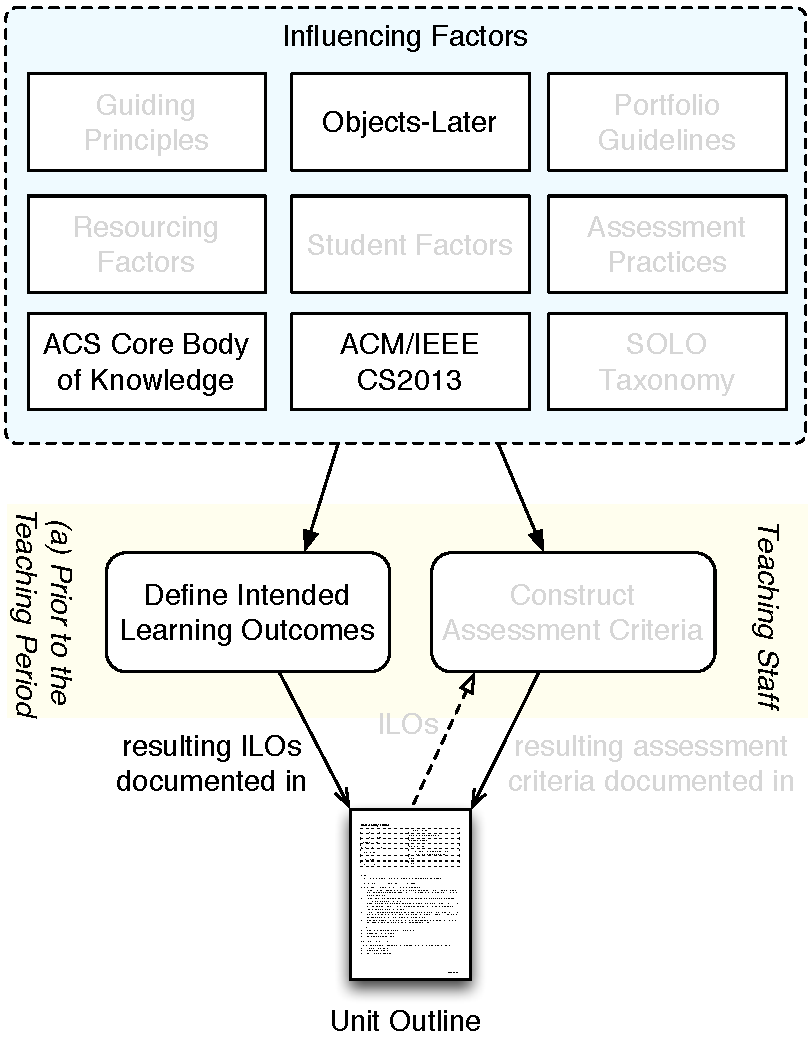
\includegraphics[width=0.7\textwidth]{ILOFactors}
	\caption{Factors that influenced the definition of the intended learning outcomes for introductory programming. \fref{fig:defining_ilos}}
	\label{fig:defining_ilos_intro}
\end{figure}

\paragraph{Objects-Later} % (fold)
\label{par:intro:objects_later}
The objects-later approach to this unit meant that it focused on structured and procedural programming concepts. The following list outlines the core concepts that were taught in this unit.

\begin{itemize}[noitemsep,nolistsep]
	\item Procedural programming abstractions:
	\begin{itemize}[noitemsep,nolistsep]
		\item Functional abstractions: functions and procedures
		\item Data abstractions: variables, constants, arrays and types
	\end{itemize}
	\item Structured programming principles:
	\begin{itemize}[noitemsep,nolistsep]
		\item Sequence, selection and repetition
		\item Control flow: pre-test and post-test loops, if and case
		\item Iteration over a collection
	\end{itemize}
	\item Program comprehension:
	\begin{itemize}[noitemsep,nolistsep]
		\item Memory layout: stack, heap and static memory
		\item Execution of control flow
		\item Parameter passing: pass-by-value and pass-by-reference
	\end{itemize}
\end{itemize}

% paragraph objects_later (end)

\paragraph{Accreditation Requirements} % (fold)
\label{par:accreditation_requirements}

The Australian Computer Society (ACS) documented the ICT profession and associated body of knowledge \cite{Gregor:2008}, which indicated graduates should develop both skills and knowledge as part of their undergraduate education. In the work, the skills component drew upon the Skills Framework for the Information Age (SFIA) while the knowledge area was divided into three aspects: a core body of knowledge, role specific knowledge and complementary knowledge. As a central role for a range of IT degrees, the introductory programming unit developed both student's skills and knowledge.

SFIA \cite{SFIA:2011} documented a range of IT skills across six categories. In terms of the SFIA, the Introductory Programming unit aimed to contribute to the development of \emph{programming and software development skill} from the \emph{Solution development and implementation} category. SFIA ranked each skill across seven levels of responsibility, ranging from \emph{follow} to \emph{set strategy, inspire and mobilise}. Introductory programming aimed to provide significant progress towards students attaining a Level 2, \emph{assist}, standard in this skill. To achieve this level of responsibility, students needed to demonstrate the ability to design, code, test, correct, and document simple programs, and indicated that students are able to assist with the development of a larger software solution.

The ACS divides the core body of knowledge into six areas: problem solving, professional knowledge, technology building, technology resources, service management and outcomes management. Introductory programming contributed toward the development of the problem solving, professional knowledge, technology building and technology resources as outlined in the following list:
\begin{itemize}[noitemsep,nolistsep]
	\item Problem solving:
	\begin{itemize}[noitemsep,nolistsep]
		\item Students used procedural programming abstractions, and were required to explain their various roles, properties and purpose. 
		\item Students followed methods and processes for designing and modelling procedural programming solutions.
	\end{itemize}
	\item Professional knowledge:
	\begin{itemize}[noitemsep,nolistsep]
		\item Students developed general computer competencies, including the use of compilers, shell scripting and basic BASH commands.
		\item Students read briefly about the history of computing, and the ICT discipline, providing a context for procedural programming and the structured programming principles.
		\item Professionalism, and the role of reflection and life-long learning in professional behaviour was instilled in students.
		\item Students performed self assessment of their competencies, and expertise, in applying procedural programming concepts. 
		\item The emphasis on demonstrating understanding enabled students to develop their written communication skills, including both technical and personal communications.
		\item Frequent interaction with staff aimed to help students development their interpersonal skills.
	\end{itemize}
	\item Technology building:
	\begin{itemize}[noitemsep,nolistsep]
		\item Students experienced many aspects of the software development lifecycle: undertaking simple analysis, design, implementation and testing processes.
		\item Students worked with iterative software development processes, building larger solutions across a number of iterations.
		\item The procedural programming topics listed above developed practical technology building skills.
		\item An understanding of the structured programming principles helped guide program construction and evaluation.
		\item Students used simple white box testing techniques to determine the success of their programs.
	\end{itemize}
	\item Technology resources:
	\begin{itemize}[noitemsep,nolistsep]
		\item Students developed a basic understanding of software systems, including the basics of software processes, memory layout and file systems.
	\end{itemize}
\end{itemize}

% paragraph accreditation_requirements (end)

\paragraph{Industry Requirements} % (fold)
\label{par:industry_requirements}

The Association for Computing Machinery (ACM) and IEEE Computer Society 2013 Computer Science Curriculum \cite{CSC2013} outlines a number of areas to be covered in a Computer Science curriculum. In terms of the ACM/IEEE model curriculum, the introductory programming unit primarily focused on \emph{Software Development Fundamentals}, but also integrated a number of other areas, as shown in the following list.

\begin{itemize}[noitemsep,nolistsep]
	\item Algorithms and Complexity:
	\begin{itemize}[noitemsep,nolistsep]
		\item \emph{Algorithmic Strategies}: students were introduced to divide-and-conquer, and the idea of recursive backtracking.
		\item \emph{Fundamental Data Structures and Algorithms}: all students programmed simple numeric algorithms, sequential search, and basic sorting.
	\end{itemize}

	\item Computational Science:
	\begin{itemize}[noitemsep,nolistsep]
		\item \emph{Processing}: fundamental programming concepts were covered in depth including algorithms,  implementing algorithms in code, and processes in the software development lifecycle.
	\end{itemize}

	\item Discrete Structures:
	\begin{itemize}[noitemsep,nolistsep]
		\item \emph{Basic Logic}: students used truth tables to learn to evaluate and construct boolean expressions.
	\end{itemize}
	
	\item Graphics and Visualisation:
	\begin{itemize}[noitemsep,nolistsep]
		\item \emph{Fundamental Concepts}: applications of computer graphics, double buffering and animation were covered to make programming more interactive.
		\item \emph{Geometric Modelling}: Optional tasks allowed students to explore procedurally generated models (fractals).
	\end{itemize}

	\item Human-Computer Interaction
	\begin{itemize}[noitemsep,nolistsep]
		\item \emph{Programming Interactive Systems}: students developed code to manage events and user interactions.
	\end{itemize}

	\item Programming Languages:
	\begin{itemize}[noitemsep,nolistsep]
		\item \emph{Basic Type Systems}: students explored the use of a range of basic types, along with the definition of custom enumerated and record types.
		\item \emph{Language Translation and Execution}: students are introduced to the topics of compilers and interpreters, as well as run-time layout of memory (call-stack, heap, static data), and manual memory management.
	\end{itemize}

	\item Software Development Fundamentals
	\begin{itemize}[noitemsep,nolistsep]
		\item \emph{Algorithms and Design}: students were introduced to the concept of algorithms, problem solving using divide-and-conquer, abstraction and program decomposition.
		\item \emph{Fundamental Programming Concepts}: students used programming language syntax, develop programs that contained statements, expressions, use variables, simple input and output operations, with conditional control flow, included functions, various parameter passing techniques, and were introduced to the concept of recursion.
		\item \emph{Fundamental Data Structures}: programs students implemented made use of arrays, record structures, strings and basic string processing, and students implemented a simple linked list.
		\item \emph{Development Methods}: program comprehension was central to the unit, with basic details of program correctness being introduced. Students were also required to use basic refactoring techniques to restructure code, and program tracing was covered as a debugging technique.
	\end{itemize}

	\item Software Engineering
	\begin{itemize}[noitemsep,nolistsep]
		\item \emph{Software Processes}: students used an iterative software development process model, and were introduced to the phases of the software development lifecycle. 
		\item \emph{Software Design}: students were introduced to the principles of the structured design paradigm, and used these principles in the design and development of the programs they created.
		\item \emph{Software Construction}: coding standards, and defensive coding practices were introduced to students.
	\end{itemize}

	\item Social Issues and Professional Practice:
	\begin{itemize}[noitemsep,nolistsep]
		\item \emph{Professional Ethics}: students develop skills in professional practice including self assessment, reflective practice, computer fluency, and general approach to life-long learning.
		\item \emph{Professional Communication}: to demonstrate their understanding students were required to read, understand and communicate technical material using clear language and visual mediums.
	\end{itemize}

\end{itemize}

% paragraph industry_requirements (end)

% subsubsection influencing_factors (end)

\subsubsection{Intended Learning Outcomes} % (fold)
\label{ssub:intro_intended_learning_outcomes}

All of the factors listed above, and those from \cref{cha:approach}, guided the definition of the intended learning outcomes for introductory programming. Given the wide range of skills and knowledge mentioned above, the challenge was to ensure that this could be expressed in a small number of intended learning outcomes. This task was assisted by the use of the SOLO taxonomy, and recognising that the SOLO level of each outcome indicated that earlier levels must already have been achieved.

The final statement of the intended learning outcomes for introductory programming are listed below, with the verbs from the SOLO taxonomy highlighted.
\begin{enumerate}[noitemsep,nolistsep]
	\item \textbf{Apply} code reading and debugging techniques to \textbf{analyse}, \textbf{interpret}, and \textbf{describe} the purpose of program code, and \textbf{locate} within this code errors in syntax, logic, and/or good practice.
	\item \textbf{Describe} the principles of structured programming, \textbf{relate} these to the syntactical elements of the programming language used, and the way programs are developed using this language.
	\item \textbf{Construct} small programs, using the programming languages covered that include the use of arrays, functions and procedures, parameter passing with pass-by-value and pass-by-reference, custom data types, and pointers.
	\item \textbf{Use} modular and functional decomposition to break problems down functionally, \textbf{represent} the resulting structures diagrammatically, and \textbf{implement} the structure in code as functions and procedures.
\end{enumerate}

Introductory programming used a procedures-first approach, and focused on the structured programming principles of organising code using \emph{sequence}, \emph{selection} and \emph{repetition}. Students learnt to use functional and modular decomposition to break problems down, and implement solutions using functions and procedures. Data was managed using arrays and custom data types. Pointers and memory management were introduced. Various forms of parameter passing were covered, including pass-by-value and pass-by-reference. Weaved through this was an iterative development process, a focus on writing clear and legible code, and other good programming practices. In addition to writing code, students learnt to read code for the debugging purposes, and to demonstrate their ability to interpret other peoples code.

Each outcome aims to engage students in activities that will help them achieve a \emph{relational} level of understanding. The verbs \emph{analyse}, \emph{apply}, \emph{construct}, \emph{implement}, \emph{interpret} and \emph{use} represent activities in which students will need to use cognitive activities that will help them achieve a relational level of understanding. The multistructural \emph{describe} verb and the unistructural \emph{locate} verb are also used, but as a supporting activity for a higher level verb, such as with describe and relate.

Many of the factors listed above are not directly stated as intended learning outcomes, but were an important part of the delivery of the unit. The decision to not include additional factors in the intended learning outcomes was a result of ensuring a clear focus within the recommended number of items; being between four and six. The remaining factors were addressed by the means through which students achieved these intended learning outcomes. This included professional communication, software engineering methods and graphics and visualisation.

\paragraph{Professional Communication} % (fold)
\label{par:professional_communication}

Traditionally, programming units focused on assessing code outcomes. Assuming that if students could produce the code, then they understood it. Others, such as \citet{Lister:2004}, have extended this to include small code reading and tracing tasks in order to expand on the assessment of student's understanding of code. With this introductory programming unit this is taken further, with the students needing to write about the associated principles and to describe code. This expanded assessment had the dual benefit of engaging higher levels of cognitive activity, while also helping students to develop their professional communication skills.

Each of the intended learning outcomes requires students to communicate their understanding. For example, in meeting the first outcome students needed to demonstrate the ability to interpret supplied code, and to communicate its purpose and any issues in logic or the application of recommended good practice. While not a direct focus of the assessment, communication skills play an enabling role in achieving this, and students were provided with support and encouragement in developing their communication skills alongside their technical skills.

% paragraph professional_communication (end)
 
\paragraph{Software Engineering Methods} % (fold)
\label{par:software_engineering_methods}

While typically the focus of later software engineering units, the software development lifecycle and iterative development methods were embedded within the unit. Students engaged in the development of software throughout the unit: analysing, designing, developing and testing software became a means for them to achieve these outcomes. Students experienced the software development lifecycle first hand, without needing it to be stated in the unit's intended learning outcomes.

Larger programs in the unit were broken down into a number of iterations, and students build these solutions by performing these iterations. Once again, this enabled them to experience software development methods without these methods being explicitly included in the assessed outcomes.

Together, both of these aspects were related to the more general concept of \emph{problem decomposition}. The idea of approaching a solution through discrete iterations provided an example of decomposing a problem into smaller steps. Similarly, the idea of breaking each of these steps into more manageable processes was used to explain both the idea of decomposition and the software development lifecycle. 

% paragraph software_engineering_methods (end)

\paragraph{Graphics and Visualisation} % (fold)
\label{par:graphics_and_visualisation}

Identifying appropriate applications for student to develop is a common problem with teaching introductory programming. In teaching introductory programming it was decided to focus on having students program small computer games. The research literature related to the use of games indicates that this is popular with students, and helps motivate them to spend time on the task, as shown in the following list.

\begin{itemize}[noitemsep,nolistsep]
	\item \citet{Roberts:1995} used a graphical library in teaching introductory programming and reported that it enhanced student interest and reinforced essential programming concepts.

	\item \citet{Feldgen:2004} reported their highest class attendance for the unit after shifting to using games, with improvements in pass rates and student retention.

	\item The greenfoot environment, introduced in \citet{Kulling:2005}, was created to help introduce high school students to object oriented programming.

	\item \cite{Rajaravivarma:2005} used text based and numeric games as a domain for introductory programming and indicated the approach created a ``passion to want to do more''.

	\item \citet{Bayliss:2006} discussed the use of games in a summer distance unit introducing students to programming and concepts in computer science. The work reported that a large percentage of students enjoyed learning introductory programming concepts in the context of games.

	\item Results from \citet{Cliburn:2006} suggested that for a large majority of students games had provided psychological motivation and had increased unit enjoyment.

	\item \citet{Leutenegger:2007} reported that games had improved student understanding of all basic topics examined.

	\item \citet{Sung:2009} provided some guidelines on incorporating games into introductory programming. This indicated an need to ensure tools are freely available, that core concepts need to remain the focus, and that games should aim to be gender and expertise neutral.

	\item \citet{Sung:2011} introduced game-themed programming assignments to help teaching staff make the transition to game based introductory programming.

\end{itemize}

The use of games as a context for software development requires students to gain some familiarity with fundamental concepts related to graphics and animation. The interactive nature of these games also introduces students to the concept of programming in response to user input events.

% paragraph graphics_and_visualisation (end)

\subsection{Constructing Assessment Criteria} % (fold)
\label{sub:intro_constructing_assessment_criteria}

The construction of the assessment criteria happened alongside the definition of the intended learning outcomes. The goal here, as stated in \cref{cha:approach}, was to create clearly distinct grades where each grade required students to demonstrate a better understanding of software development. 

\fref{fig:assessment_criteria} shows the assessment criteria for the introductory programming unit. Each of the grades uses the levels discussed in \cref{cha:approach}. For \emph{Pass} and \emph{Credit} students completed the set exercises, which were only signed off through student interaction with staff. \emph{Distinction} required the implementation of a program of the student's own creation, which \emph{High Distinction} required a small research project.

\begin{figure}[htbp]
	\centering
	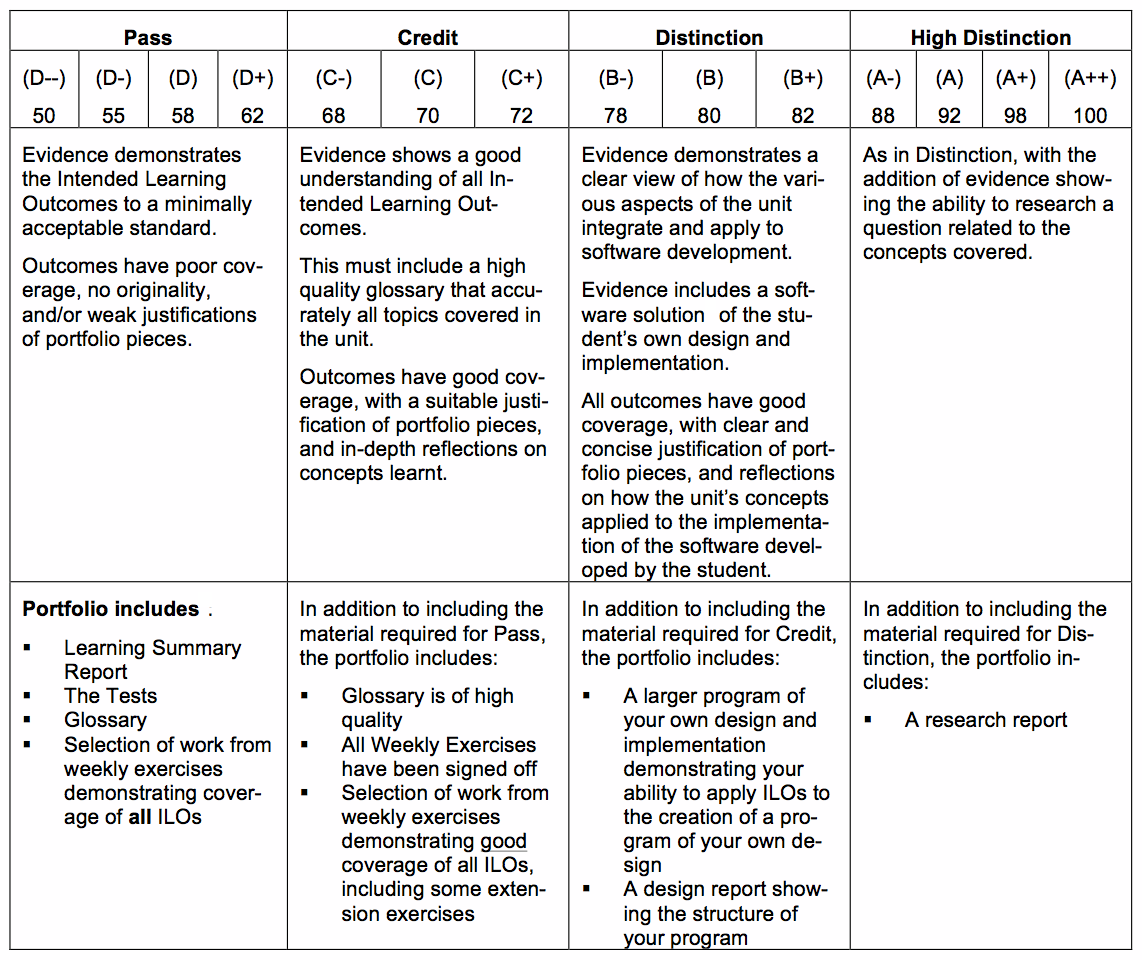
\includegraphics[width=\textwidth]{AssessmentCriteria}
	\caption{The assessment criteria from the Unit Outline of the introductory programming unit.}
	\label{fig:assessment_criteria}
\end{figure}

To receive at least a Pass grade, students needed to satisfactorily complete three hurdle tests as well as including a number of pieces of work that demonstrated they had met all of the intended learning outcomes. These pieces of work needed to work from the weekly tasks, but did not need to have been signed off by teaching staff. 

The \emph{Credit} grade required students to meet all pass requirements, and to have succeeded in getting all tasks signed off. This ensured we were happy they had completed the work themselves and providing them with incentives to engage in the formative feedback process. Their explanation of programming concepts and abstractions, in their Glossaries, was the main item to distinguish between Pass and Credit in terms of depth of understanding. In this regard, the student's glossary needed to demonstrate good coverage of all outcomes for the student to be eligible for a Credit grade.

\emph{Distinction} built on top of the Credit requirements and required students to create a program of their own design. This could be any program the student was interested in creating, as long as it demonstrated good coverage of all of the unit's intended learning outcomes. In effect, this meant that students needed to create a program that contained a number of functions and procedures, used arrays and record types, and was of sufficient size and complexity. Most students who received this grade had implemented a game of some kind, many emulating classic arcade games such as asteroids, pong, frogger or space invaders.

\emph{High Distinction} required students to engage in the creation of a short research report, in addition to having met the Distinction grade requirements. Each student aiming to achieve this grade worked together with staff to define a topic they could examine, and then the student carried out data collection, analysis and reporting tasks. As an introductory programming unit, this research was limited to examining simple tasks such as algorithm efficiency, different techniques to perform a task, or comparing performance aspects of different code. Students were encouraged to think deeply about their results, and to document their outcomes clearly.

% subsection constructing_assessment_criteria (end)

\subsection{Developing Teaching and Learning Activities} % (fold)
\label{sub:intro_developing_teaching_and_learning_activities}

Allocated classes for the introductory programming unit included a two hour lecture, and a two hour laboratory class each week, over a thirteen week teaching period. All classes were designed with the goal of actively engaging students. A typical lecture included a short presentation using ``Beyond Bullet Points'' style lecture slides \cite{Atkinson:2007}, an interactive programming demonstration and group activities. In the laboratory sessions, students were involved in code reading activities, guided programming tasks and practical hands-on exercises.

The teaching period consisted of thirteen weeks, twelve of which were teaching weeks, and a single week semester break. Topics for the twelve lectures are shown in the following list. In weeks one to six students explored these concepts using a modern version of the Pascal programming language \cite{Wirth:1971,FPC:2011}. In week 7 students were introduced to the C programming language \cite{Ritchie:1978}, which was used for the remainder of the semester. 

\begin{enumerate}[noitemsep,nolistsep]
  \item Programs, Procedure, Compiling and Syntax
  \item User Input and Working with Data
  \item Control Flow: Branches and Loops
  \item Procedural and Structured Programming
  \item Arrays
  \item Custom Data Types and Pointers
  \item Learning a New Language
  \item Programming in C
  \item File Input and Output
  \item Dynamic Memory Management
  \item Recursion and Backtracking
  \item Review and Future Studies
\end{enumerate}

\subsubsection{Lecture Slides} % (fold)
\label{ssub:lecture_slides}

The concept-based approach discussed in \cref{cha:approach} guided the choice to use the ``Beyond Bullet Points'' style lecture slides \cite{Atkinson:2007}. This approach is draws upon the work on Richard Mayer (see \citet{Mayer:2005}), and structures presentations using a storyboard approach. The structure of the storyboard is shown in \fref{fig:bbp}.

\begin{figure}[htbp]
	\centering
	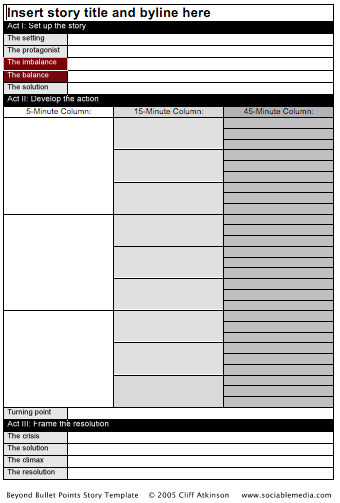
\includegraphics[width=0.95\textwidth]{bbp}
	\caption{Storyboard template from \url{http://beyondbulletpoints.com} outlining the stages in a Beyond Bullet Points presentation.}
	\label{fig:bbp}
\end{figure}

Students are guided through the first five slides that set up the ``story'', telling the audience why they are there and centring them as the main character in the story. This helps motivate the discussion, and focused the teaching staff on clearly communicating the motivation behind the topic being presented. The first five slides contain the following details:
\begin{enumerate}[noitemsep,nolistsep]
	\item The first slide sets the \emph{context}, positing the story at a relevant place within the content of the unit.
	\item The \emph{protagonist} slide indicates the story is about them, they are the focus not the teaching staff.
	\item Slide three indicates the \emph{imbalance}, stating a current problem, challenge or opportunity.
	\item Juxtaposing slide three, slide four presents the situation in which the problem or challenge has been addressed, or the opportunity has been realised. This is the \emph{balance} slide.
	\item This leaves slide five to present our \emph{solution}, indicating how students (the main character) can get from the current imbalance to the desired balance.
\end{enumerate}

The of these slides contained a full sentence, written in an active voice. Ideally they can be accompanied by visuals to set a theme or metaphor for the presentation. The time and resources necessary for this was seen as contrary to \pref{itm:agile}, being agile and willing to change these teaching and learning activities. Instead, a minimalist approach was taken and these slides clearly showed the sentence text.

For a fifteen minute presentation, the body of the presentation contained three main points, supported by three sub-points. Each addressed a ``why'' or ``how'' point, and supported the main solution. Once again these required a single short sentence in an active voice. The composition of these slides usually drew upon visuals created as part of the teaching and learning resources for the unit.

The last five slides conclude the presentation, reminding students of the overall solution and the new balance it brings about. These slides contain the following details:
\begin{enumerate}[noitemsep,nolistsep]
	\item The first slide in the conclusion was the \emph{turning point}. This is a question that asks a question of the students, indicating the presentation has turned to the conclusion. In effect it asks them if the concepts presented have shown them how to address the imbalance from the introduction.
	\item Next the \emph{crisis} slide restates the balance and imbalance, reminding the students of where the presentation started and where it was aiming to go.
	\item This then leads nicely to a restating of the \emph{solution}. This is an exact duplicate of the solution from the introduction, but now the student have been though the ``story'' and it should have more meaning.
	\item The \emph{climax} brings all of the pieces of the story together in summary and give the teaching staff a final opportunity to motivate students to study the topic further themselves.
	\item The final slide is the \emph{resolution}, and indicates the end of the presentation.
\end{enumerate}

Many of these guidelines from the Beyond Bullet Points approach were applied in the development of the lecture slides for the introductory programming unit. This included the general structure of the stroyboard, though in some cases the three points were stretched to four but not beyond. The body of the presentations did include some information on ``what'' can be used, rather than purely focusing on ``how'' and ``why''. The use of active sentences, and visual communication free from lists of bullet points were also applied.

By sticking as tightly to these ideas as possible the lecture presentations remained focused on concepts, with little if any syntax being included. Slides used visual representations to communicate programming concepts, and the limited number of points focused the presentation to only the most important aspects. This forced details to be communicated in other means, as will be discussed in \cref{cha:supporting}. An example of the lecture slides is shown in \fref{fig:lecture}.

\begin{figure}[htbp]
	\centering
	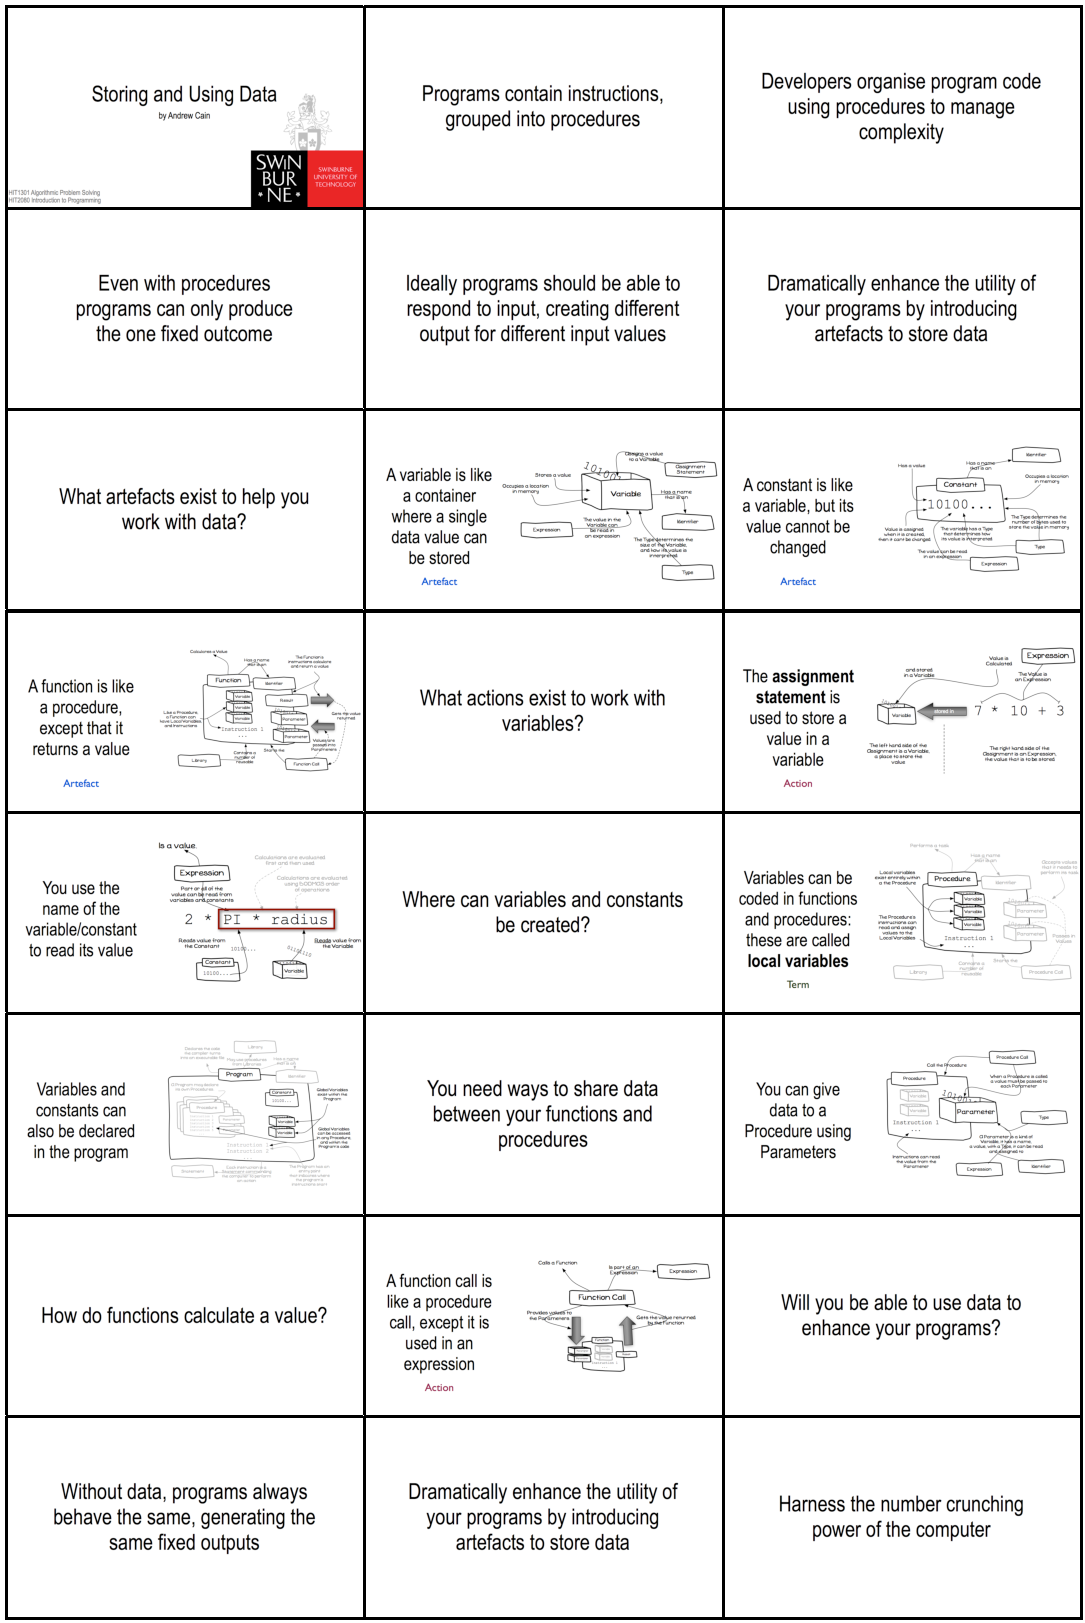
\includegraphics[width=\textwidth]{Lecture}
	\caption{Sample slides from the Topic 2 lecture on data.}
	\label{fig:lecture}
\end{figure}

% subsubsection lectures (end)

\subsubsection{Interactive Lecture Demonstrations} % (fold)
\label{ssub:interactive_lecture_demonstrations}

% subsubsection interactive_lecture_demonstrations (end)


\subsubsection{Laboratory Sessions} % (fold)
\label{ssub:laboratory_sessions}

% subsubsection laboratory_sessions (end)

\subsubsection{Programming Language Choice} % (fold)
\label{ssub:programming_language_choice}

\cite{Becker:2002}

To facilitate the shift in programming language, students were introduced to ``understanding syntax'' from week one. Students learnt to read programming language syntax using the visual ``railroad'' diagram syntax notation \cite{Braz:1990}. Each of the lecture topics focused on concepts, with syntax being offloaded to programming demonstrations and supplied notes. In the teaching and learning resources, each programming statement had an associated railroad diagram, with small code examples to illustrate its application. These resources will be discussed further in \cref{cha:supporting}.

% subsubsection programming_language_choice (end)

% subsection developing_teaching_and_learning_activities (end)



\subsection{Assessing Student Portfolios} % (fold)
\label{sub:assessing_student_portfolios}

The process for assessing student portfolios is shown in \fref{fig:assessment_process}. This involved the following steps:

\begin{enumerate}[noitemsep,nolistsep]
	\item Determine grade from the self assessment, cross referenced with data collected from the student during the teaching period.
	\item Initially assume the work meets is ``average'' within its grade, then examine evidence and self assessment to determine if the result is of a higher or lower standard than average.
	\item After completing all assessment, re-examine all students who achieve the ``top'' High Distinction grade and determine if any should be awarded a perfect score.
\end{enumerate}

\begin{figure}[htbp]
	\centering
	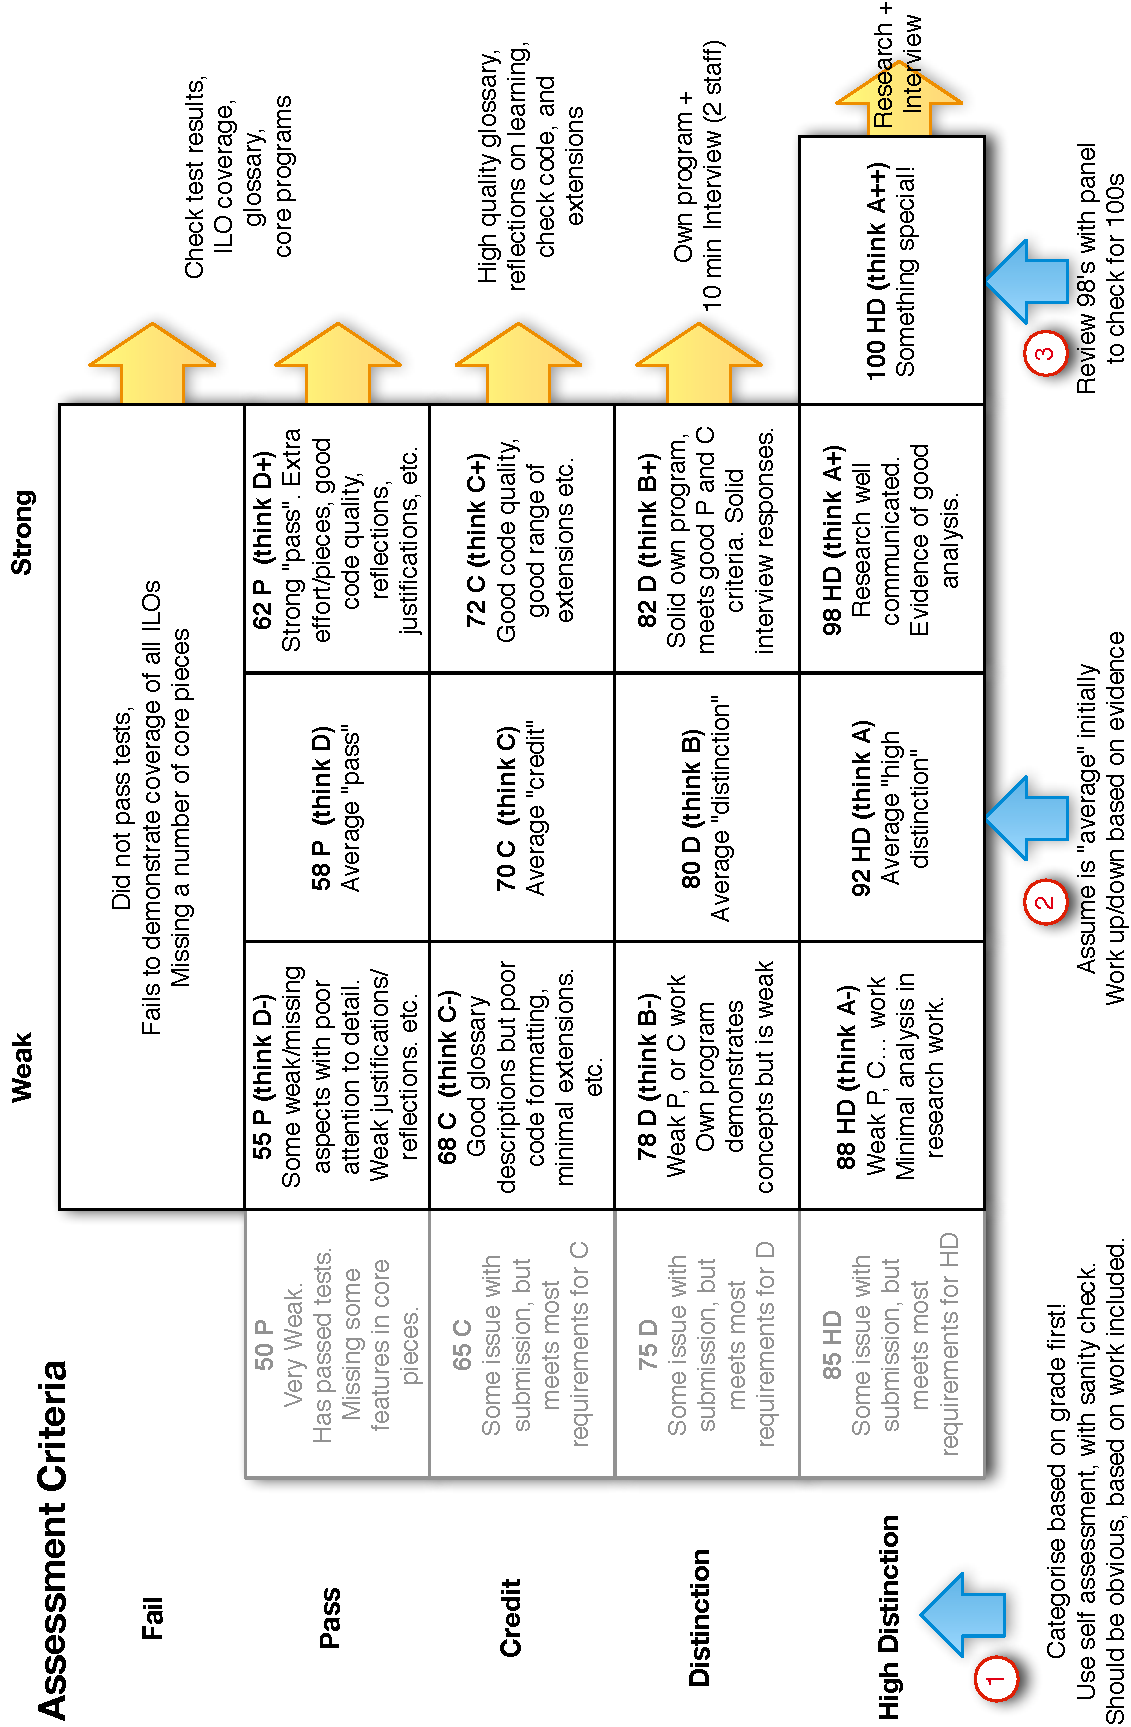
\includegraphics[width=0.98\textwidth]{AssessmentProcess}
	\caption{An overview of the assessment process used to explain the criteria to students.}
	\label{fig:assessment_process}
\end{figure}

The clearly distinct criteria for each grade make determining portfolio grades a simple task. Pass criteria required students to have satisfactorily completed the hurdle tests, Credit required a good quality glossary and all work to be signed off, Distinction the custom project and High Distinction the research report. 

For each of the grades the quality of the distinguishing artefact needed to be checked against the expected standard. In the final portfolio assessment this task was greatly simplified due to the requirement for students to engage in the formative feedback process for Credit and higher grades. This meant that student work had already been checked by teaching staff, typically a number of time, before their portfolios are even submitted. Any issues should have been identified, and corrected, before the final summative assessment.

% subsection assessing_student_portfolios (end)



% section introductory_programming (end)
\clearpage
\section{Object Oriented Programming} % (fold)
\label{sec:object_oriented_programming}




% subsection object_oriented_programming (end)

Object Oriented Programming takes students who have completed Introductory Programming and introduces them to the object oriented programming paradigm. Students will learn about the core principles of object oriented programming, and how these can be used to create object oriented programs. They will develop programs using integrated development environments, including  unit testing tools. Students will be introduced to visual ways of communicating object oriented designs using the Unified Modelling Language \cite{Fowler:2004}, including both class diagrams and sequence diagrams. Design patterns and heuristics will be used to provide students with a means of evaluating the quality of their designs. As with Introductory Programming students will use a iterative development process. The intended learning outcomes for Object Oriented Programming are:
\begin{enumerate}
	\item Explain the principles of the object oriented programming paradigm specifically including abstraction, encapsulation, inheritance and polymorphism, and explain how these principles are used to create object oriented programs.
	\item Design, develop, test, and debug object oriented programs, using an integrated development environment.
	\item Select and use appropriate collection classes, from the language's class library, to manage collections of multiple objects.
	\item Construct appropriate diagrams and textual descriptions to communicate the static structure and dynamic behaviour of an object oriented solution.
	\item Apply accepted good practices related to the construction of object oriented programs.
\end{enumerate}
% subsection intended_learning_outcomes (end)



% section concepts_in_introductory_programming (end)

\section{A Simplified Taxonomy to Frame Programming Concepts} % (fold)
\label{sec:a_simplified_taxonomy_to_frame_programming_concepts}

% section a_simplified_taxonomy_to_frame_programming_concepts (end)

\section{Introductory Programming, Procedures First} % (fold)
\label{sec:introductory_programming_procedures_first}

% section introductory_programming_procedures_first (end)

\section{Using Multiple Languages to Focus on Concepts} % (fold)
\label{sec:using_multiple_languages_to_focus_on_concepts}

% section using_multiple_languages_to_focus_on_concepts (end)

% chapter constructively_aligned_introductory_programming_curriculum (end)